\chapter{Погребальная Радунка}

Мы снова возвращаемся в Выгуровщину, на берег озера Гнилуши, прежде бывшей частью русла речки Радунки.

Речка под названием Радунка – не монополия Киева. Был еще левый приток Угры – Радунка (Руденка, Радунья).

С названием беда. Ежели корень «радун», то это вероятно указывает на происхождение от Радуницы (Родоницы) – весенними днями поминовения усопших (Гробки, Красная горка, Фомина неделя – следуют за Пасхой).

Если же корень «руд», то это значит «рыжий», а у меня из головы не выходит русло с рыжей водой, у села Выгуровщины, соединенное с Черторыей, да в окрестностях есть болотная руда. Между Радункой и Руденкой разница всего в две буквы, и Родунь начинает весьма напоминать «рудню», место добычи и выплавки железа.

Ученые полагают, что на восточном берегу озера Гнилуши стоял летописный Городец, а позже на том же месте был двор князя Симеона Олельковича. Это место – в наши дни точно не указываемое – слывет в науке «городищем». А упоминаемое в давних земельных документах урочище Селище объявлено учеными «посадом» Городка, и кажется соотносится наукой с выгоном на север от Гнилуши. Где-то в «посаде», площадь коего определена в 5 гектаров, археологи нашли черепки и разные отходы, датировав их 11-13 веками.

Сведения об изучении «городища» в советское время – отрывочны, дореволюционные – редки, но более подробны.

Рассмотрим все сообщения о предмете и сравним, сколь находки под Выгуровщиной совпадают с выводами ученых. Сыщутся ли следы летописного Городка (в летописи никак не описанного, кроме имени и общих, да противоречивых сведений об его положении) или позднейшего «замочка» Симеона Олельковича.

Поначалу сопоставление Городка и «замочка» проявлялось смутно.

В 19 веке, М. А. Максимович, явно знакомый с документами (что видно по словам «пустое городище»), писал:

\begin{quotation}
Замок киевского князя Симеона Олельковича принадлежал не к старому городу, а стоял против него на левой стороне Днепра, за Чорторыею. На месте сего замка в 17 веке было уже пустое заглохшее городище с довольно высокими валами, которое называли Олельковым городищем. За ним не в далеком расстоянии находились Сторожевые горы. Может быть на месте сего городища и в древнее время был Городец, известный в наших летописях.
\end{quotation}

Может и был, но кроме предположения нужен довод в его пользу, здесь довода нет.

Закревский в «Описании Киева» (1868), цитируя известный нам документ с ограничением земель, про борок, замок и двор князя Олельковича, пишет – мол, некоторые думают, тут и был летописный Городок.

Да вот, сколько лет прошло, а наука не ушла от мнения этих некоторых, и даже закрепила оное.

Первое печатное упоминание о «городище» при Выгуровщине, причем безо всякого исторического толкования, известно мне по книге «Древние города России» (1873) археолога Дмитрия Яковлевича Самоквасова:

% я наткнулся на двадцатью годами раннее, нежели у Завитневича, описание «городища»: 

\begin{quotation}
Остерский уезд.

Городище в Броварской волости, при селе Выгуровщине, на север, в разстоянии от села на 1/4 версты\footnote{Около четверти километра.}. Насыпь вышиною 12 аршин\footnote{8,52 метра.}, мерою вокруг на одну десятину\footnote{1,09 гектара.}, и кругом обведена канавою в четыре аршина\footnote{2,84 метра.} глубины, для входа в городище имеются признаки существовавших ворот. Д. В. Пр. №1353.

Городище в той же волости, внутри селения Выгуровщины. Такая же самая насыпь, как и предыдущая, на ней ныне существует двор Киево-Михайловского монастыря. Д. В. Пр. №1353\footnote{Эти же сведения повторены в приложении к книге Самоквасова «Северянская земля по городищам и могилам» (1908).}. Номера означают номера донесений волостных правлений. Эти донесения Самоквасов получил осенью 1872-го, попросив губернатора послать во все волости запрос о сведениях про курганы. На прилагаемой к «Северянской земле» карте городищ у Киева оранжевыми точками отмечены два «городища», одно на Вигуровщине, другое на Троещино.
\end{quotation}

Вот как. Два «городища».

«Городище» по месту села Троещино – положим, это так отметили «городище» у Гнилуши, ведь оно, как и Троещино, находились тогда к северу от обжитого пространства Выгуровщины. А может было какое-то городище и в Троещине. Это первое описанное «городище» имело высоту трехэтажного дома, да еще занимало площадь в один гектар.

Однако мы узнаём про еще одно «городище», такое же, однако внутри самой Выгуровщины!

Два сходных, по гектару, высоких городища – это следы чего-то весьма большого, и занимавшего пространство по меньшей мере двух гектаров, если поставить эти участки вместе. А ведь они были разведены на некое расстояние.

Итак, Самоквасов написал про два городища, но есть вероятность третьего – в селе Троещино. Вопросы множатся.

Можно ли сопоставить какое-либо из этих городищ со знаменитым и неуловимым «городищем» на восточном берегу Гнилуши? А на западном берегу? А с тем «городищем», которое описано в земельных грамотах?

Спустя двадцать лет, окрестности Выгуровщины стал изучать Виктор Гошкевич, сведя в соображениях своих в одну точку замок Олельковича и летописный Городок. В докладе-статье 1889 года «Замок Симеона Олельковича и летописный Городок под Киевом» он обстоятельно излагает летописные сообщения про Городец и цитирует некоторые старинные земельные документы, включая объемную часть протокола комиссии, которую водили по спорным местам.

Изложив источники, Гошкевич начинает их толковать, вооружившись картой Шуберта. Я не согласен с толкованиями Гошкевича, однако приводить их не буду по другой причине – не хочу запутывать свою книгу. Например, Черторыя и Десна у Гошкевича одно и то же – Десной он называет Черторыю вдоль Троещины и Выгуровщины, и тут же рядом именует сие русло Черторыей. Чтобы войти в мир представлений Гошкевича полностью, нужно полностью прочесть его статью.

Я же сделаю из нее выдержки.

В «толкованиях» Гошкевич приводит важные для меня сведения. Так, он говорит, что от «вилообразного» водоема, который «тянется через с. Вигуровщину» (значит, речь идет о Прудке, хотя Гошкевич полагает описываемый им водоем частью остатков Гнилуши) «вытекает болотистый ручеек и впадает в третье озеро, прилегающее с запада к с. Воскресенскому» (следовательно, от Прудка к озеру Радунке при Гошкевиче тянулся ручеек).

%Затем Гошкевич отмечает «далее по старинному руслу Гнилуши сохранилось лишь несколько маленьких озерец, в виде многоточия идущих на юг до Цепного моста, где Гнилуша впадала в устье Черторыи». Это те самые озерца по впадине, что тянется ниже озера Радунки. 

%По Гошкевичу, речка Гнилуша это нынешние озеро Гнилуша, Прудок, озеро Радунка, и озера ниже. Я таких выводов сделать не смог, низовье документированной речки Гнилуши ускользает от меня.

%Речка Радунка, по его словам, «должна быть признана за восточный приток Десны. Выходила она из Десны у с. Троещины, огибала его, поворачивала к югу и текла параллельно Черторые, снова впадая в Десну несколько ниже с. Вигуровщины».

«Борок» из документов, по Гошкевичу, 

\begin{quotation}
песчаная возвышенность, поросшая сосновым лесом, почти примыкающая к Вигуровщине с северовосточной стороны. Нынешние размеры этого борка по длине не превышаю 2 верст (от севера к югу), а по ширине – 1 версту (от востока к западу.
\end{quotation}

Полагаю, с «борком» Гошкевич сопоставил некий сосновый лесок конца 19 века, вероятно где сейчас улица Деснянская. Другой возвышенность там просто нет, кроме еще берега озера Гнилуши.

Городище же Гошкевич относит к северо-западу от Вигуровщины (в границах конца 19 века), «на левом берегу речки Гнилуши, между этой речкой и борком».

%«Старое кладовище», коего комиссия 18 века не могла найти, ибо даже тогда это было название урочища, места, а не кладбища с покойниками, Гошкевич отождествляет с кладбищем 19 века «вблизи северного конца Вигуровщины», а кладовище новое, осмотренное комиссией, «находилось у опушки бора, ближе к Троещине». Так сгинувшее много веков назад урочище возродилось у Гошкевича в буквальном своем назначении!

В статье Гошкевич подробно рассказывает о краеведческой вылазке, предпринятой на основе размышлений над документами:

\begin{quotation}
Имея такое подробное определение местности, отправился я, вместе с В. З. Завитневичем, 13 сентября для осмотра замчища. Разыскать же его, имея в руках трехверстную карт, оказалось делом вовсе не трудным.

От Никольской слободки, что у цепного моста, мы пошли по дороге к с. Воскресенскому, мимо длинного узкого озера\footnote{Конечно же, озеро Радунка.}, составляющего часть русла старинной речки Гнилуши. Из расспросов окрестных жителей оказалось, что озеро это теперь не носит особого имени, а зовется, как и село, Воскресенским\footnote{Однако на картах есть название Радунка, и улица в слободке именовалась Радонковской.}.

Дорога на Вигуровщину идет отсюда по берегу ручья, который также особого названия, кажется, не имеет. Ручей привел нас к длинному озеру, по обеим сторонам которого расположена Вигуровщина\footnote{Вероятно Прудок. Ибо только по его обоим берегам была расположена Выгуровщина. Что до озера Гнилуши, то у него ныне населен только восточный берег.}.

Озеро это, конечно, также часть старого русла речки Гнилуши; крестьяне называют его Михайловским, по имени киевского монастыря, который и поныне владеет как самым озером, так и землями у Вигуровщины.

Мы прошли мимо «дворца монастырского», расположенного невдалеке от приходской церкви, на возвышенном месте: это деревянное двухэтажное здание с мезонином, почерневшее от времени\footnote{То ли, 18 века, упомянутое комиссией? Вспомним и сведения Самоквасова, что одно из городищ занято монастырским двором.}. 

При выходе из села мы сразу ступили на песчаную почву; вправо, на песчаных буграх группами расположены сосны – это опушка борка. 

Тут же, у опушки леса, виднеются на на песке следы давнишней жизни человека: масса черепков от разбитых глиняных сосудов, валяются человеческие кости. Назвать это место «старым кладовище» или «селищем», которые упоминаются в приведенных актах, кажется, нет основания, судя по положению этого места, сравнительно с другими, упоминаемыми в тех же актах.

Под бором и в самом бору идет теперь оживленная работа: вигуровщане строят здесь на возвышенности свои хаты, во избежание весенних разливов.

Расспросив крестьян, как пройти к речке, которую они же назвали Гнилушей, мы направились по болотистой долине, примыкающей к озеру Михайловскому, по опушке леса. Долина эта, несомненно, составляет также старинное русло Гнилуши, которая, как видно из показания Василия Закгуры, рыбалки стародавнего, жителя киевского, еще в начале XVIII века «взялася з Старика Днепра, а упадала в озеро Михайловское»\footnote{Гошкевич ссылается на «связку документов Михайловского монастыря, лист 135, номер 137, опись 209». Значит, упорядоченные Петровым документы из архива Киевской Духовной Академии попали в библиотеку Вернадского.}.

Сосны в бору гигантские; мы смеряли одно дерево, растущее над долиною: окружность его у основания оказалась в 5 1/3 аршин\footnote{3,8 метра.}. Это – живой, но безмолвный свидетель раздоров монахов из-за поля Чуриловского, и побития городничего Иакинфа.

Все идя по-над долиною, мы подошли к высоким валам городища князя Симеона Олельковича: тылом городище обращено к бору, находясь от него в расстоянии нескольких десятков саженей, а с противоположной стороны оно примыкает к речке Гнилуше, то есть тому озерцу, которое на карте имеет форму прямого угла\footnote{Имело, на карте Шуберта. Стало быть, Гошкевич говорит о том, что ныне известно как озеро Гнилуша, примыкающее к западной окраине села Выгуровщины.}.

Если провести прямую линию между церквами Вигуровской и Троещинской, то линия эта пересечет городище\footnote{По карте Шуберта (где село Троещина стоит на другом месте, нежели при Гошкевиче), или на местности в 1899 году?}.

Вал, окружающий городище, сохранился прекрасно: он имеет подкововидную форму, отверстием к Гнилуше, то есть по направлению к Киеву. Длина вала 130 саженей; поперечник от одного конца подковы до другого – 67 саженей; перпендикулярный к нему – 43 сажени\footnote{277,  143, 92 метра.}. Высота вала от уровня воды в Гнилуше – 3 сажени\footnote{6,4 метра.}.

Явственно сохранились старинные въезды в городище: один с северо-запада, а другой с юго-востока. Кажется, что городище было обведено еще и другим валом, меньшей высоты.

Поверхность городища покрыта песчаными буграми; по всему городищу, особенно же в южной его части, лежат прямо на поверхности тысячи обломков глиняной посуды, попадаются массивные глиняные ушки от каких-то больших сосудов, железные гвозди, жужелица.

По словам окрестных жителей, на городище находят металлические крестики и «карбованцы»; в одном месте, по их же рассказам, есть в городище обширный провал, глубину которого они меряли когда-то шестом\footnote{Значит, опасались спуститься туда сами, а дно не просматривалось.}.

У берега Гнилуши вал обвалился, и здесь, на глубине 2 1/3 аршин\footnote{1,4 метра.} от поверхности, залегает горизонтальный слой угля, толщиною вершков в 6\footnote{4,26 метра.}, а из-под него выглядывают черепа и другие человеческие кости. Мы вынули полуистлевшую детскую головку, рядом с которой торчали кости взрослого человека.

Скелеты находились в гробах, остатки коих, со вбитыми в них гвоздями, виднеются рядом с костями на склоне обрыва\footnote{Гошкевич примечает: «О существовании здесь городища находим краткое упоминание в III томе Записок Археологического института». Что же за городище и замок Олельковича такое, когда полно мертвецов?}.

Слой угля, лежащий под верхнею насыпью городища, приводит к мысли, что на том же месте, где во второй половине XV века стоял двор и замок кн. Симеона Олельковича, существовало более древнее поселение, истребленное огнем, – а кн. Симеон засыпал пожарище толстым слоем глины и сам поселился на старом пепелище.
\end{quotation}

Мысль ученых на этот счет, кажется, не изменилась по сей день.

Во время своей краеведческой вылазки с Завитневичем, Гошкевич совершил поверхностный осмотр местности, и я благодарен за подробное описание. Впрочем из этого описания уже проступает нечто странное – какие-то покойники, гробы... Больше похоже на давнее кладбище, нежели остатки «замочка» или более древнего поселения.

По одному только описанию Гошкевича нельзя вычислить место «городища». Ведь если идти сейчас вдоль берега Гнилуши, между нею и селом, никаких следов вала и гектарного возвышения (кроме возвышения самого берега) не заметишь. Не видать их и севернее, в поле, где огороды и выгон. На восточном берегу Гнилуши, куда Гошкевич помещает «городище», нынче всё застроено частными домами и что-либо осмотреть невозможно.

Спустя год, профессор Киевской Духовной Академии Владимир Зенонович Завитневич\footnote{Завитневич (1853-1927) – церковный и светский историк, археолог, богослов, публицист. Похоронен на Щекавицком кладбище, на уничтоженной ныне его части.} вернулся к Выгуровщине, провел там раскопки и описал их в работе, почти одноименной со статьей Гошкевича – «Замок князя Семена Олельковича и летописный Городец под Киевом»\cite{zavit01}.

%Завитневич описал свои раскопки и черпал данные из одноименной, предшествующей работы знакомого своего, В. И. Гошкевича «Замок князя Симеона Олельковича и летописный Городец под Киевом» (Труды Киевск. Дух. Акад. 1890. Февраль. 228-254), в которой по земельным документам вычислялось место замка Олельковича и Городца. Завитневич, принимавший участие в краеведческих вылазках Гошкевича, провел раскопки этого «городища». 

%Скудные сведения о нем помещены и в «Своде памятников Украины». На плане Сноевского оно подписано просто «Городище». Соберу данные об этом месте воедино, но вначале опишу состояние местности на 2014 год.

Что же обнаружил Василий Зенонович? Я буду широко цитировать его статью, она редкая – и вам полезно, и мне меньше пересказывать.

На раскопки у Завитневича ушло три дня, с 29 по 31 мая 1890 года. Впрочем он называет раскопки пробными. Проведены они были по предложению Императорской Археологической Комиссии. В статье дается карта и следующее описание.

\begin{quotation}
Настоящее городище расположено к северу от деревни Вигуровщины, на восточном берегу продолговатаго озера, представляющаго остаток русла речки Гнилуши, составлявшей рукав р. Черторыи. 
\end{quotation}

Увы, я не располагаю картой, где была бы показана Выгуровщина в 1890 году. На плане Шуберта середины 19 века застройка еще не доползла до широты озера Гнилуши, и окраина села лежит к югу от окончания озера. На плане 1914 года застройка дошла с юга до половины озера.

Указание «к северу от деревни Вигуровщины» должно трактоваться с привязкой к тогдашнему состоянию застройки. Без этого и дополнительных указаний в статье, можно предполагать городище по всей длине Гнилуши, на восточном ее берегу.

\begin{quotation}
Форма городища – почти правильный полукруг, примыкающий открытою стороною к озеру. Вокруг вала видны следы глубокаго когда-то рва, теперь по местам почти совершенно занесеннаго песком. Длина вала 390 арш.; длина линии, соединяющей концы полукруга 201 арш.; длина линии, опущенной перпендикуляром к последней от средины вала, т.е. широта городища в центре 129 арш\footnote{277,4 метра; 143 метра; 91,74 метров.}. Отвесная высота насыпи вала не везде одинакова; южный конец подымается на 2,5 арш. над почвенным слоем; северный – на 1 арш.; средняя часть вала – на 2 арш. и 12 верш.; широта насыпи у основания средним числом равняется 28 арш.\footnote{1,8 метра; 0,71 метров; 1,94 метра; 19,9 метров.}
\end{quotation}

\begin{center}
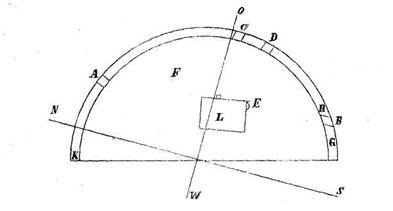
\includegraphics[width=\linewidth]{chast-gorodki/radunka/zavitn.jpg}
\end{center}

\begin{quotation}
Для выхода из городища есть два прохода: один с северной (А) стороны, другой с южной (В); оба, повидимому, современны первоначальному образованию вала. Кроме того с восточной стороны вал имеет две выемки, одна значительная (С), другая малозаметная (В); но обе они образовались уже на памяти местных обывателей путем действия ветра на песчаную насыпь вала. 

Топография внутренней части городища обусловливается характером берега озера, на котором оно расположено. Восточный берег озера в направлении с севера на юг постепенно повышается, подымаясь в южной части городища до 5,5 арш.\footnote{3,9 метра.} над уровнем воды в озере. Сообразно с этим южная площадь городища возвышенна, северная – низменна. Южная возвышенная часть городища прорезана по линии АВ продолговатым углублением, образовавшимся, повидимому, вследствие искони существовавшаго здесь прохода и проезда. Северная часть городища настолько низменна, что во время весенняго половодия нередко заливается водою из озера.

Последнее обстоятельство по всей вероятности было причиною того, что древние обитатели этого городка воздвигали свои постройки только в северной его части, в чем можно убедиться на основании сохранившагося здесь мусора, представляющаго следы человеческаго жилья.
\end{quotation}

Почему археологи и историки чаще всего составляют карты с произвольным направлением, и пририсовывают потом стрелку с юга на север? Не проще ли всю карту строить так, чтобы север оказался наверху?

Озеро на карте примерно там, где линия NS (север-юг). Описываемый Завитневичем вал – он отмечен на карте полукругом – находился не вдоль береговой линии, а проходил по нынешнему частному сектору.

Продолжу знакомить вас с наиболее важными кусками статьи Завитневича:

\begin{quotation}
Южная оконечность вала представляла крутой обрыв, при обвалах котораго обнаруживались человеческие костяки в гробах. Это обстоятельство заставило меня прежде всего обследовать южную оконечность вала до прохода В.

Предназначенная для раскопки площадь (G) имела по длине вала 16 арш., в ширину 22,5 арш.\footnote{11.4 метра и 16 метров.} Площадь эта предварительно окопана была со всех сторон траншеями, при помощи которых определена была линия, обозначившая границу между нетронутым почвенным слоем и верхнею насыпью. При послойном снимании насыпи вала в обозначенных траншеями пределах найден был 21 костяк, из которых 10 было детских; остальные принадлежали взрослым людям. Все покойники похоронены были в деревянных гробах; гробы находились в насыпи на различной высоте; большая часть их помещена была в центральной части вала, на глубине 0,5 аршина\footnote{0,35 метра.} от поверхности насыпи; другие лежали на самом почвенном слое. Никаких предметов при костях не найдено. Сравнительно хорошая сохранность костяков не позволяет относить их к глубокой древности.
\end{quotation}

Если я верно понимаю, судя по высоте берега и соотнося ее с современным рельефом, захоронения были в районе западной части улицы Довженко и северной улицы Димитрова. Эти улицы пересекаются почти около современного южного конца Гнилуши.

Всего в ста метрах к востоку от этих гробов лежит Выгуровское кладбище. Может, это всё – древняя погребальная местность?

Кажется весьма странным, что гробы были закопаны в насыпном валу, полукругом. Усматриваю в этом нечто обрядное. Местность «городища» ограждена покойниками, они в гробах своих стерегут внутреннюю область между валом и озером.

Еще в который раз замечу, как обыденно археологи разоряют древние кладбища.

Но вот что пишет Завитневич пишет далее:

\begin{quotation}
Под насыпью, на почвенном слое, оказалось огнище. Начинаясь в центре, оно наполняло собою весь юго-восточный угол отведенной для изследования площади и находилось, кажется, на самом возвышенном пункте озернаго берега. Огнище это, мало походило на те кострища, с которыми археологам приходится встречаться в курганах с трупо-сожжением: оно было следствием действия сильнаго и продолжительнаго огня. О силе огня можно заключать из того, что многие предметы не только медные, но и железные, совершенно разложились и, смешавшись с песком, образовали целыя труды безформеннаго сплава. 

Что этот сплав образовался путем воздействия огня на металлические предметы, имевшие определенную форму, это видно из таких остатков, как медная пряжка, несколько таких же пластинок и остаток, повидимому, раковидной медной фибулы\footnote{Фибулой на ученом языке называют застёжку, обычно украшенную с той или иной долей затейливости. Слово «застёжка», по мнению ученых, звучит антинаучно.}. В центре кострища находилось небольшое овальной формы углубление, вымазанное красной глиной и служившее, кажется, местом раскладки огня. Что это место служило чем-то в роде жаровни, это видно из того, что не только красная глина, но и находившийся, под нею толстый слой илистаго чернозема, превратились от действия огня в твердый как камень кирпич.

Но непосредственное действие огня не ограничивалось этим пунктом; оно обнимало довольно широкую площадь, вся поверхность которой при вскрытии с трудом поддавалась ударам заступа. В составлявшем кострище мусоре явно можно было отличить куски древеснаго угля, кости больших животных, скорлупу от яйца и следы некоторых других органических предметов.

Но в то время, когда одна часть рабочих, находясь на верху насыпи, снимала ее горизонтальными слоями, другая часть, работая в боковых траншеях, раскапывала ту же насыпь вертикальными слоями, приближаясь таким образом от периферии к центру. Последний способ раскопки дал возможность констатировать следующий факт.

Под насыпью вала, ниже уровня земли, обнаружено было еще несколько костяков; но здесь покойники погребены были в то время, когда насыпи вала еще не было: вертикальныя линии, обозначавшия границы могил, подымались здесь лишь до известнаго уровня, затем прекращались.

При вертикальном разрезе насыпи казалось, как будто бы гробы поставлены были на свои места с боку, они как будто задвинуты были в проделанныя с боку ниши.

Таким образом в истории настоящаго кладбища можно отметить две эпохи: первая – до образования искусственной насыпи вала, вторая – после образования последней.

Не лишне будет отметить и следующий факт. Костяки обоих кладбищ, т.е. верхняго и нижняго, принадлежали покойникам арийскаго племени; но в обряде их погребения замечена следующая разница: покойники нижняго кладбища хоронились в особаго рода войлочных шапках, известных на юго-западе России под именем «шеломков»; в обряде же погребения покойников верхняго кладбища ничего подобнаго не замечено. В свою очередь, по отношению к последним можно отметить то, что они погребались в особаго рода кожаных башмаках, известных под названием «кожанцов».

Кроме того в одном из гробов нижняго кладбища найдена лишь верхняя часть человеческаго костяка без ног; в другом гробу оказалось две головы, лобная часть в одной из которых пробита, повидимому, каким то тупым орудием.

Настоящая раскопка обнаружила таким образом тот факт, что южная оконечность вала искони служила местом кладбища. Теперь естественно возникал вопрос: ограничивалась ли кладбищенская часть площадью G, или она простиралась по ту сторону прохода B в пределы площади H? Чтобы решить этот вопрос, необходимо было перенести изследование по другую сторону прохода B, что и сделано было много. 

Стена вала, ограничивавшая проход B с востока (H) изследована была путем прорытия во всю ширину вала траншеи шириною в 3 аршина\footnote{2,13 метра.}. На этом пространстве обнаружено было 9 гробов, которые точно также находились на различной высоте: одни помещались в насыпи вала, другие опускались на несколько вершков (до 9)\footnote{40 сантиметров.} ниже поверхности земли. 

Но особеннаго внимания заслуживает следующий факт. В самой насыпи здесь обнаружено, так сказать, два яруса: верхний и нижний; при чем замечено было, что некоторые из гробов опускались в землю в то время, когда верхняго яруса насыпи еще не существовало. Из этого видно, что вал разсматриваемаго городища насыпан был, по крайней мере в некоторых местах, в два приема и следовательно в истории его следует различать две эпохи – древнейшую и новейшую. 

Этот факт мною отчасти подмечен был и при изследовании площади G, но там он выступал не так рельефно. Кроме того мною произведено было изследование в проходе C и в северной оконечности вала (K). Но в этих пунктах ни гробов, ни двух-яруснаго состава насыпи вала не было обнаружено.

Из этого следует, что верхний ярус насыпи образовался при ремонте вала, которому подверглись лишь некоторыя его части. [...]

Приступая к изследованию внутренней части городища, я предварительно приказал прорыть в разных местах несколько пробных ям. Посредством этих ям выяснилось, что культурный слой, состоящий из перегноя, из котораго ветром и дождем выносятся разнаго рода предметы, самой большей толщины достигает в границах площади L. Площадь эта, длиною (с севера на юг) в 20 арш. и шириною (с востока на запад) в 18 арш.\footnote{Длина 14,2 метров, ширина 12,8.}, окопана была глубокими траншеями и затем поверхность ея, на глубине культурнаго слоя, снималась очень тонкими пластами; при этом обнаружилось, что культурный слой, начинаясь в западной части очень тонким пластом, самой большей толщины достигал в югозападной части площади L, где глубина его доходила до 1,5 арш.\footnote{1,06 метра.} 

На всем этом пространстве прежде всего попадались черепки от битой посуды и кости больших и малых домашних животных. Посуда, насколько можно судить на основании сохранившихся черепков, приготовлена была на гончарных станках, из хорошей различнаго цвета глины. Что касается формы посуды и попадающагося на некоторых черепках орнамента, то в них нет ничего типичнаго, настолько характернаго, чтобы их можно было относить к той или другой определенной эпохе.

Из других предметов при изследовании данной площади найдены были: железный топор древняго славянскаго типа; шесть железных стрел, из которых пять копьевидных и одна якоревидная, с двумя зазубнями и втулкой для надевания на древко; несколько небольших железных ножиков, на подобие тех, которые попадаются в славянских курганах, небольшия ножницы того типа, который и теперь употребляется для стрижки овец, куски железных тонких обручей для оковки ведер такого типа, с которым приходится встречаться в славянских курганах, несколько общеизвестных шиферных пряслиц; два колечка: одно из тонкой медной проволоки без спайки, другое из какого-то составнаго металла, сделанное в подражание витым кольцам; оба кольца принадлежат к типу, с которым приходится встречаться в курганах; железный ручной браслет, железная иголка, небольшая медная бубенчиковидная пуговка, небольшой нательный орнаментированный крестик, и несколько других железных предметов; точно определить назначение которых затруднительно.

Путем сопоставления предметов, добываемых из курганов, с такими же предметами несомненно позднейшаго происхождения, в настоящее время доказана удивительная устойчивость форм многих предметов домашнего обихода. В виду этого весьма трудно сказать, к какой именно эпохе относится все вышепоименованные предметы. Всего вероятнее то, что здесь мы имеем дело с наслоениями нескольких эпох.
\end{quotation}

Что же сообщил Завитневич? Из его статьи я выпустил разве что рассуждения о том, что это место летописного Городца и позже – замка Симеона Олельковича. Мне важны данные. 

Данные таковы. Найдено весьма странное сооружение – погребальный полукруглый вал. Под валом – тоже могилы. Стало быть, сначала полукругом хоронили в земле, потом был насыпан вал, и захоронения продолжились уже в нем. Слыхано ли такое дело?

Между валом и берегом озера археолог нашел не следы построек, а мусор – черепки, кости, да металлические мелочи, частью вероятно поганского времени.

Вырисовывается следующая картина. Берег речки Радунки, на нем – полукруглая площадка, огражденная погребальным валом. Это не место жительства, это нечто другое. Место поклонения? Может потому и называлась местность Радосынь, а речка Радункой – от «радения»? Радение значит молитвенные песни, религиозные пляски. А праздник Радуница – день памяти покойников, когда у могил радовались, плясали да пели.

Но праздновали Радуницу на обычных кладбищах, а тут особое. Полукругом да в несколько ярусов.

Ниже по течению речки Радунки, у нынешнего озера Радунки или Радужного – знаменитая, теперь позабытая, левобережная Лысая гора. Лысые горы представляются мне местами, где прежде, в языческие времена, совершались различные обряды – после принятия христианства их вынуждены были отправлять уже тайно, а в народе они прослыли шабашами.

В пяти километрах к северо-восток от Выгуровщины лежит село Погребы, в чьем названии можно усмотреть тот же корень, что у слова «погребение».

Любопытно проследить другие название сёл, лежащих оттуда на север вдоль древнего (а частью современного) русла Десны. За Погребами – Зазимье, потом Пуховка, затем Рожевка. Тут колокольчик позвонил у меня в голове, напомнив о поклонении Славян Рожаницам. А к северу от Рожевки лежит село... Рожны. Неспроста!

Но вернемся к Выгуровщине. 

Про раскопки тут Сагайдака я ничего не знаю, кроме того, что они проводились в 1990 году. После Завитневича, «городище» изучал ленинградский археолог П. А. Раппопорт, о чем он поведал в статье «Исследования городищ в районе Киева в 1950 году», опубликованной в 7-м томе украинского журнала «Археология» за 1952 год.

Приведу оттуда выдержки, переводя с украинского на русский.

\begin{quotation}
Городище размещено на северной околице с. Выгуровщина, на берегу небольшого озера, которое представляет собой остатки пересохшей речки Гнилуша. Городище окружено валом, который имеет в плане почти правильную полукруглую форму и своими концами упирается в береговую террасу р. Гнилуша. Высота этой террасы около 5 м.
\end{quotation}

Раппопорт приводит план «городища» на 1950 год, ориентированный на север, однако без какой-либо привязки к окружающей местности:

\begin{center}
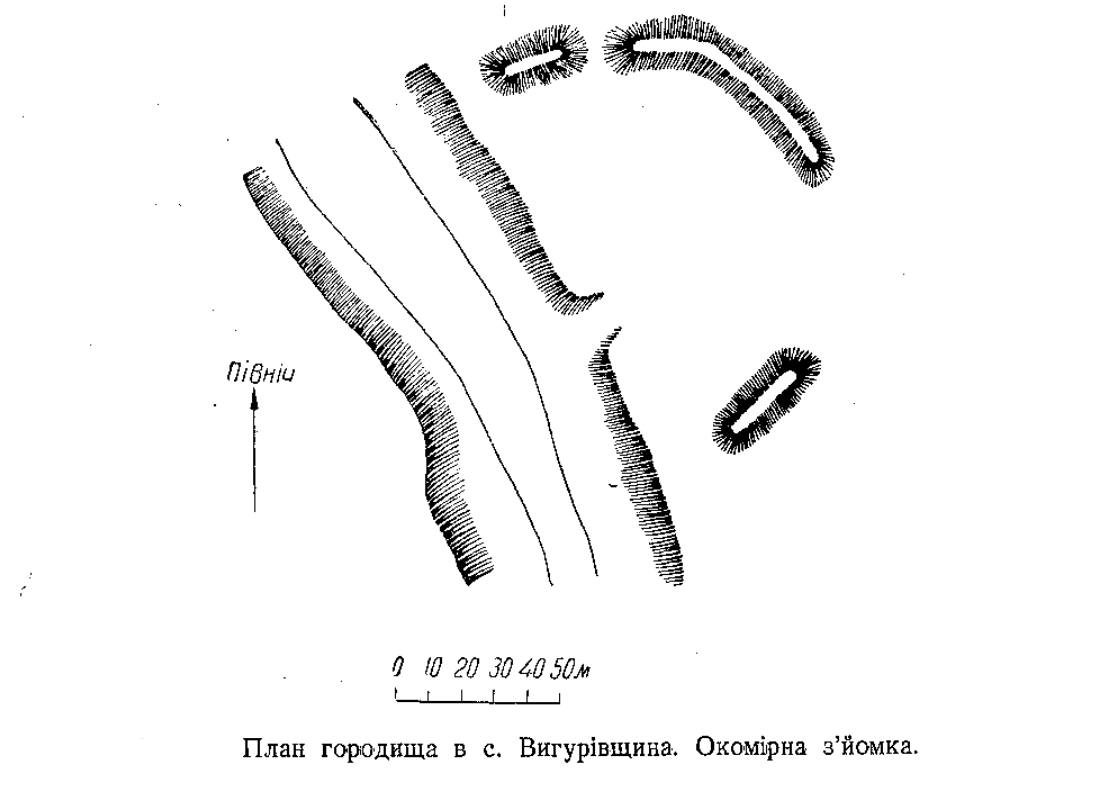
\includegraphics[width=\linewidth]{chast-gorodki/radunka/rapp.jpg}
\end{center}

И продолжает:

\begin{quotation}
Вал городища сохранился лишь в виде трех отдельных участков. Высота вала в некоторых местах достигает 3 м. В северной части городища перед валом видно остатки рва глубиной всего около 0,7 м. Площадка посреди городища примерно на 0,7 м выше окружающей территории. Площадь городища 120х80 м.

Прорезка северного участка вала городища показала, что этот вал состоит из светложелтого лессоподобного суглинка и представляет собой не искусственную насыпь, а только подправленную холмистость местности. Исходя из раскопок 1890 г., в южной части городища вал состоял из насыпной земли. Таким образом, система обороны этого городища состояла из использованной как вал складки местности, дополненной насыпным валом.
\end{quotation}

Стоп!

Какая система обороны?! Погребальный вал, где гробы с покойниками лежат ярусами.

\begin{quotation}
На север от городища было расположено селище, которое на основании обнаруженного материала, как и городище, можно датировать XI-XIII веками. Городище, очевидно, представляет собой остатки города Городец, который упоминается в древнерусских летописях в XI-XII веках.
\end{quotation}

Вот и всё что в статье сказано о «городище». Что за «селище», что именно нашли – неясно. Про Олельковичей однако ни слова. Про похоронное назначение вала – тоже. 

Полагаю, на север от погребального вала просто нашли следы обжитости этой местности в давние времена. Сколь далеко простирались эти следы – ну как раскопали, 5 гектаров из заметки в «Своде памятников».

У меня совсем другое представление об окрестностях Выгуровщины, чем у науки. Я не знаю, какими соображениями она руководствуется. Разве на берегу Гнилуши найдены остатки построек какого-либо двора, «замочка»? Или раннего Городка?

Нет! Вал, нашпигованный в несколько ярусов гробами! И следы металлургической деятельности внутри полукруга вала.

На основании источников, я представляю себе в древности большое обжитое пространство вдоль реки Радунки, где кроме прочего на берегу стоял этот загадочный погребальный вал.

Странно это – русло, к нему примыкает полукруг с мертвецами. Место со стороны Гнилуши, а значит реки Радунки – открытое. В древности вы бы сошли допустим с лодки и, поднявшись на небольшой пригорок, оказались внутри полукруга этого вала. И там же, внутри, что-то делали с огнем и металлом. Священное место, посещаемое с берега? Место проведения обрядов?

Я пробовал найти упоминания о чем-то подобном в других местах. Нет, нигде не прятали гробы в полукругом валу и под валом. Это не вписывается ни в один известный мне погребальный обряд. Нечто особенное для Киева.

Казалось бы, вот загадка, отечественный Стоунхэндж. Ученые – решайте! 

Нет, они повторяют, что здесь было городище замка Олельковича, а попутно летописный Городец.

Насколько соотносится указанное в старинных документах «городище Олелковича» с этим похоронным сооружением? Оба были на берегу Гнилуши, неясно впрочем на каком было «городище», но допустим, что на том же, где и вал – на восточном.

На некоторых современных картах урочище Городище (описанный мною выгон) отмечается к северу от застроенного места проведенных Завитневичем близ Гнилуши раскопок. Участок выгона, судя по всему, пустовало веками.

Но и место «городища» на берегу нынешнего озера Гнилуши тоже не застраивалось, кажется, до 20 века.

Городище Олельковича документально освещено как сгинувшее, просто как место былого поселения, двора, имения княжеского. Нет ни жалованных грамот про него как про живое и существующее. Оно возникает отголоском, призраком прошлого, «городищем пустым». Отчего пустое? Тут рядом монастыри рвут друг другу глотки за каждый клочок земли, но городище, да еще на выгодной возвышенности, куда не достает в половодье вода – пустое.

А в самом ли деле где-то там было городище двора Олельковича? Или так с каких-то пор стали называть, без оснований на то, место полукруглого погребального вала?

А как называли два или три городища, описанные Самоквасовым, и как соотнести их с упомянутыми в земельных документах? Ну «северное городище» можно соотнести с погребальным валом у берега Гнилуши. А как быть с городищем, что Самоквасов поместил внутри самой Выгуровщины?

Добавим к этому городище (не знаю, верно ли его так называть), заметное на западном берегу Гнилуши.

Выходит, целых три «городища» на Выгуровщине да при ней, из коих одно является странным погребальным валом. Уместно предположить, что вся тройка это части чего-то большого, что  раскинулось по обе стороны бывшей реки Радунки, а существование вала с захоронениями должно как-то вписываться в общую картину, будучи лишь ее составляющей. Что же такое изображала вся картина?

Добавим еще один штрих.
